\documentclass{article}

% Preamble
\usepackage[margin=0.7in]{geometry}
\usepackage{amssymb}
\usepackage{mathrsfs}
\usepackage{amsmath}
\usepackage{mathtools}
\usepackage{graphicx}
\usepackage{listings}
\usepackage{xcolor}
\usepackage{enumitem}
\usepackage[colorlinks=true, linkcolor=blue, urlcolor=blue]{hyperref}
\usepackage{float}
\usepackage{minted}

\definecolor{codegreen}{rgb}{0,0.6,0}
\definecolor{codegray}{rgb}{0.5,0.5,0.5}
\definecolor{codepurple}{rgb}{0.58,0,0.82}
\definecolor{backcolour}{rgb}{0.95,0.95,0.92}

\lstdefinestyle{mystyle}{
    backgroundcolor=\color{backcolour},   
    commentstyle=\color{codegreen},
    keywordstyle=\color{magenta},
    numberstyle=\tiny\color{codegray},
    stringstyle=\color{codepurple},
    basicstyle=\ttfamily\footnotesize,
    breakatwhitespace=false,         
    breaklines=true,                 
    captionpos=b,                    
    keepspaces=true,                 
    numbers=left,                    
    numbersep=5pt,                  
    showspaces=false,                
    showstringspaces=false,
    showtabs=false,                  
    tabsize=2
}

\lstset{style=mystyle}
\renewcommand{\familydefault}{\sfdefault}
\hyphenpenalty=10000

\title{Project 8 Report}
\author{Nathan Hutton}
\date{}

\begin{document}

\maketitle

First I just rendered a red plane:\\
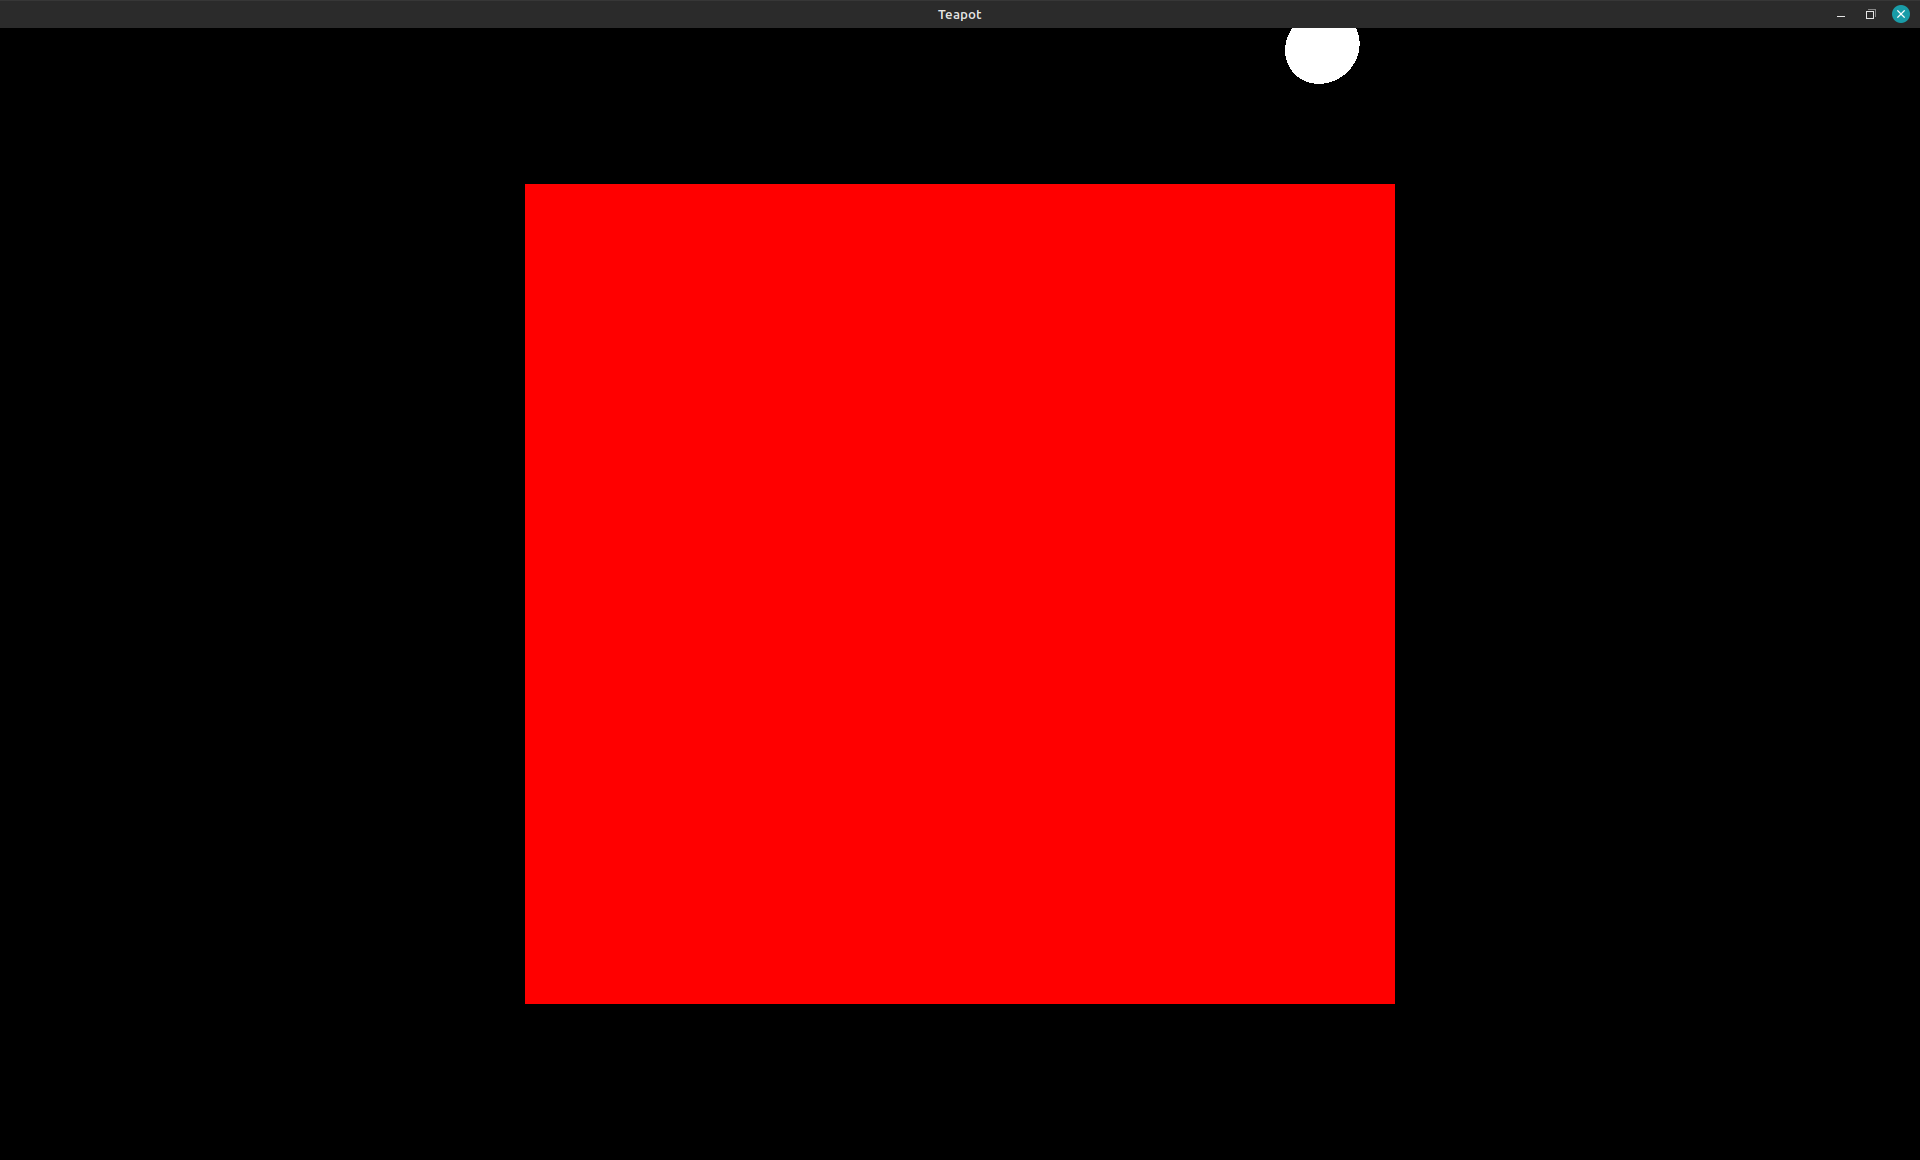
\includegraphics[width=0.7\textwidth]{images/redPlane.png}\\
I kept the spotlight representation there for now since I'd need it later.\\[2mm]
Next I got normal mapping working:\\
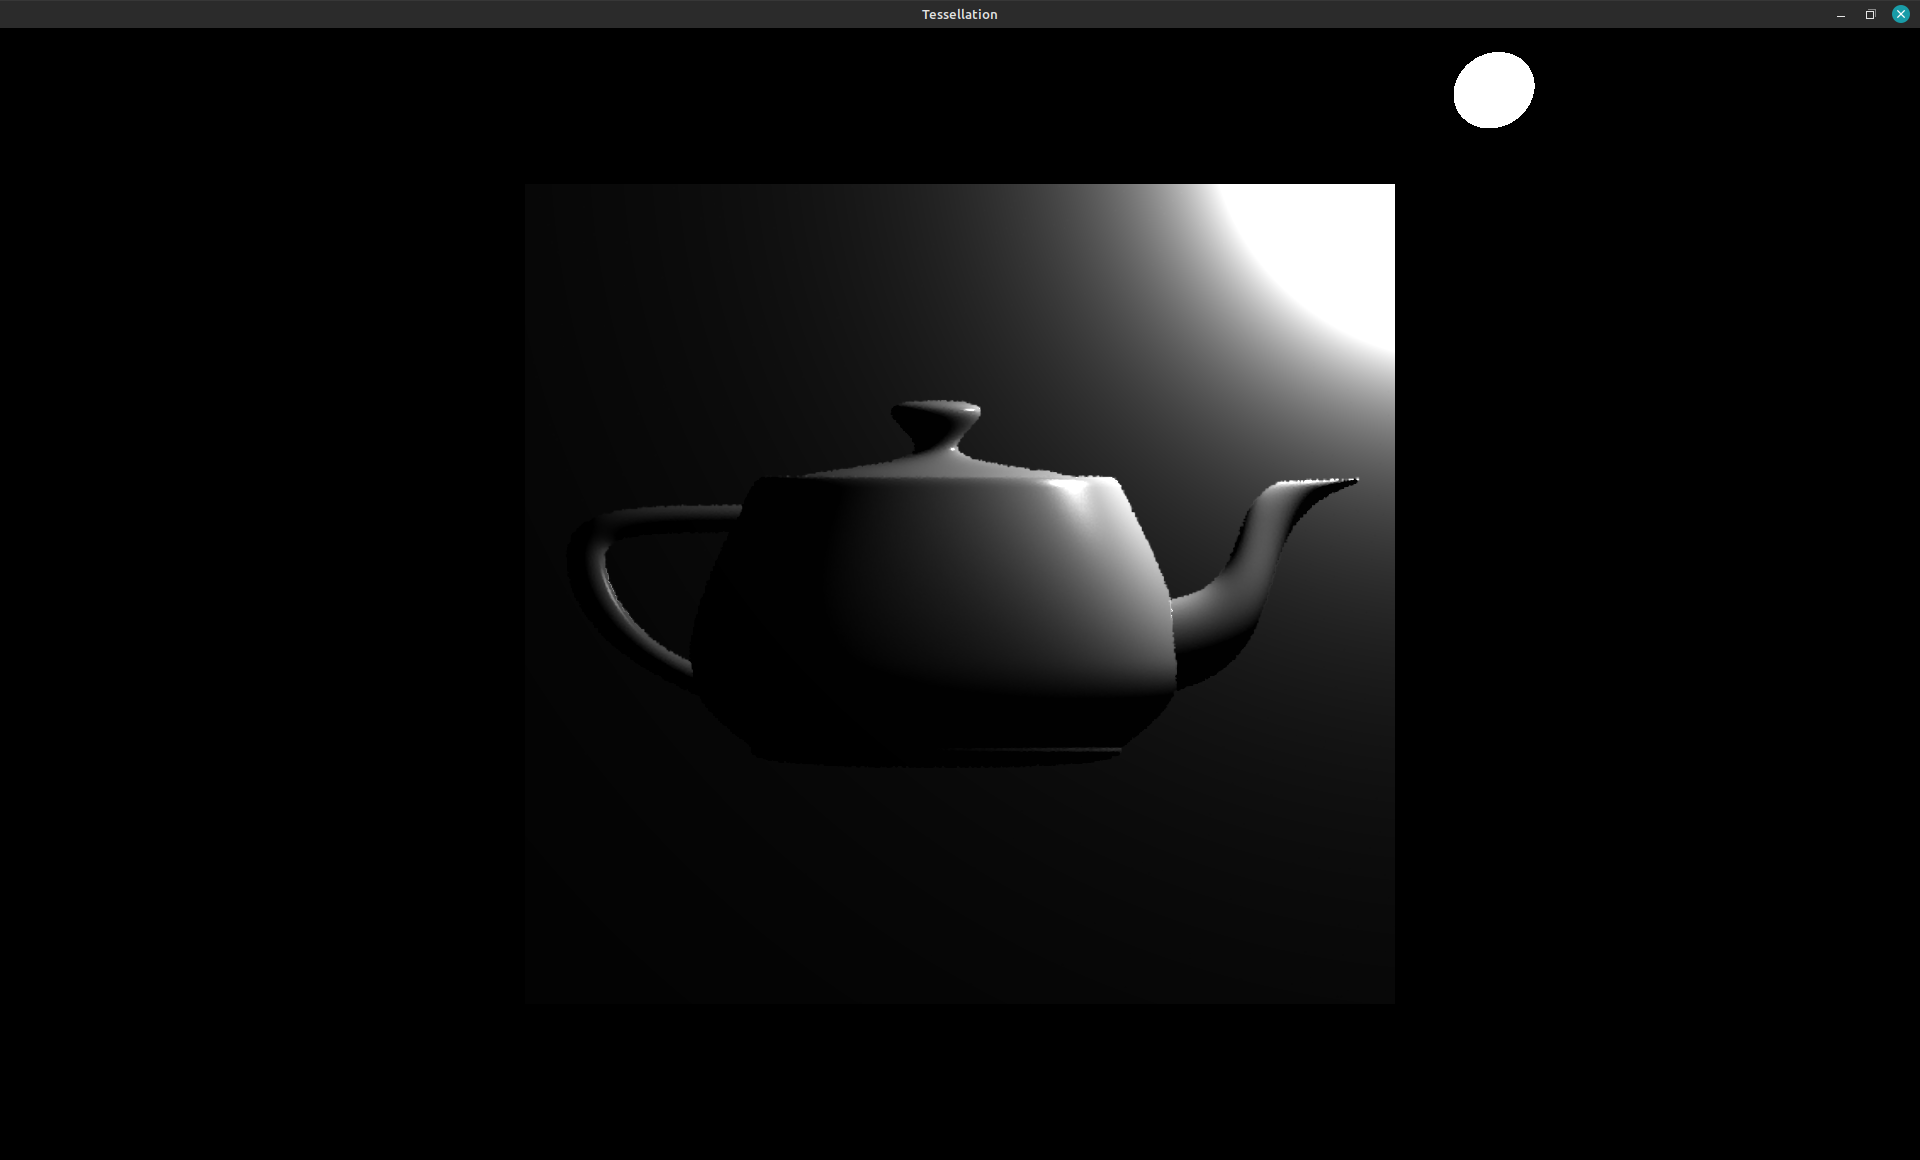
\includegraphics[width=0.7\textwidth]{images/normalMap.png}\\
For some reason I needed to flip the y texture coordinate to get the teapot to not be flipped across the x-axis.\\
Next I did triangulation:\\
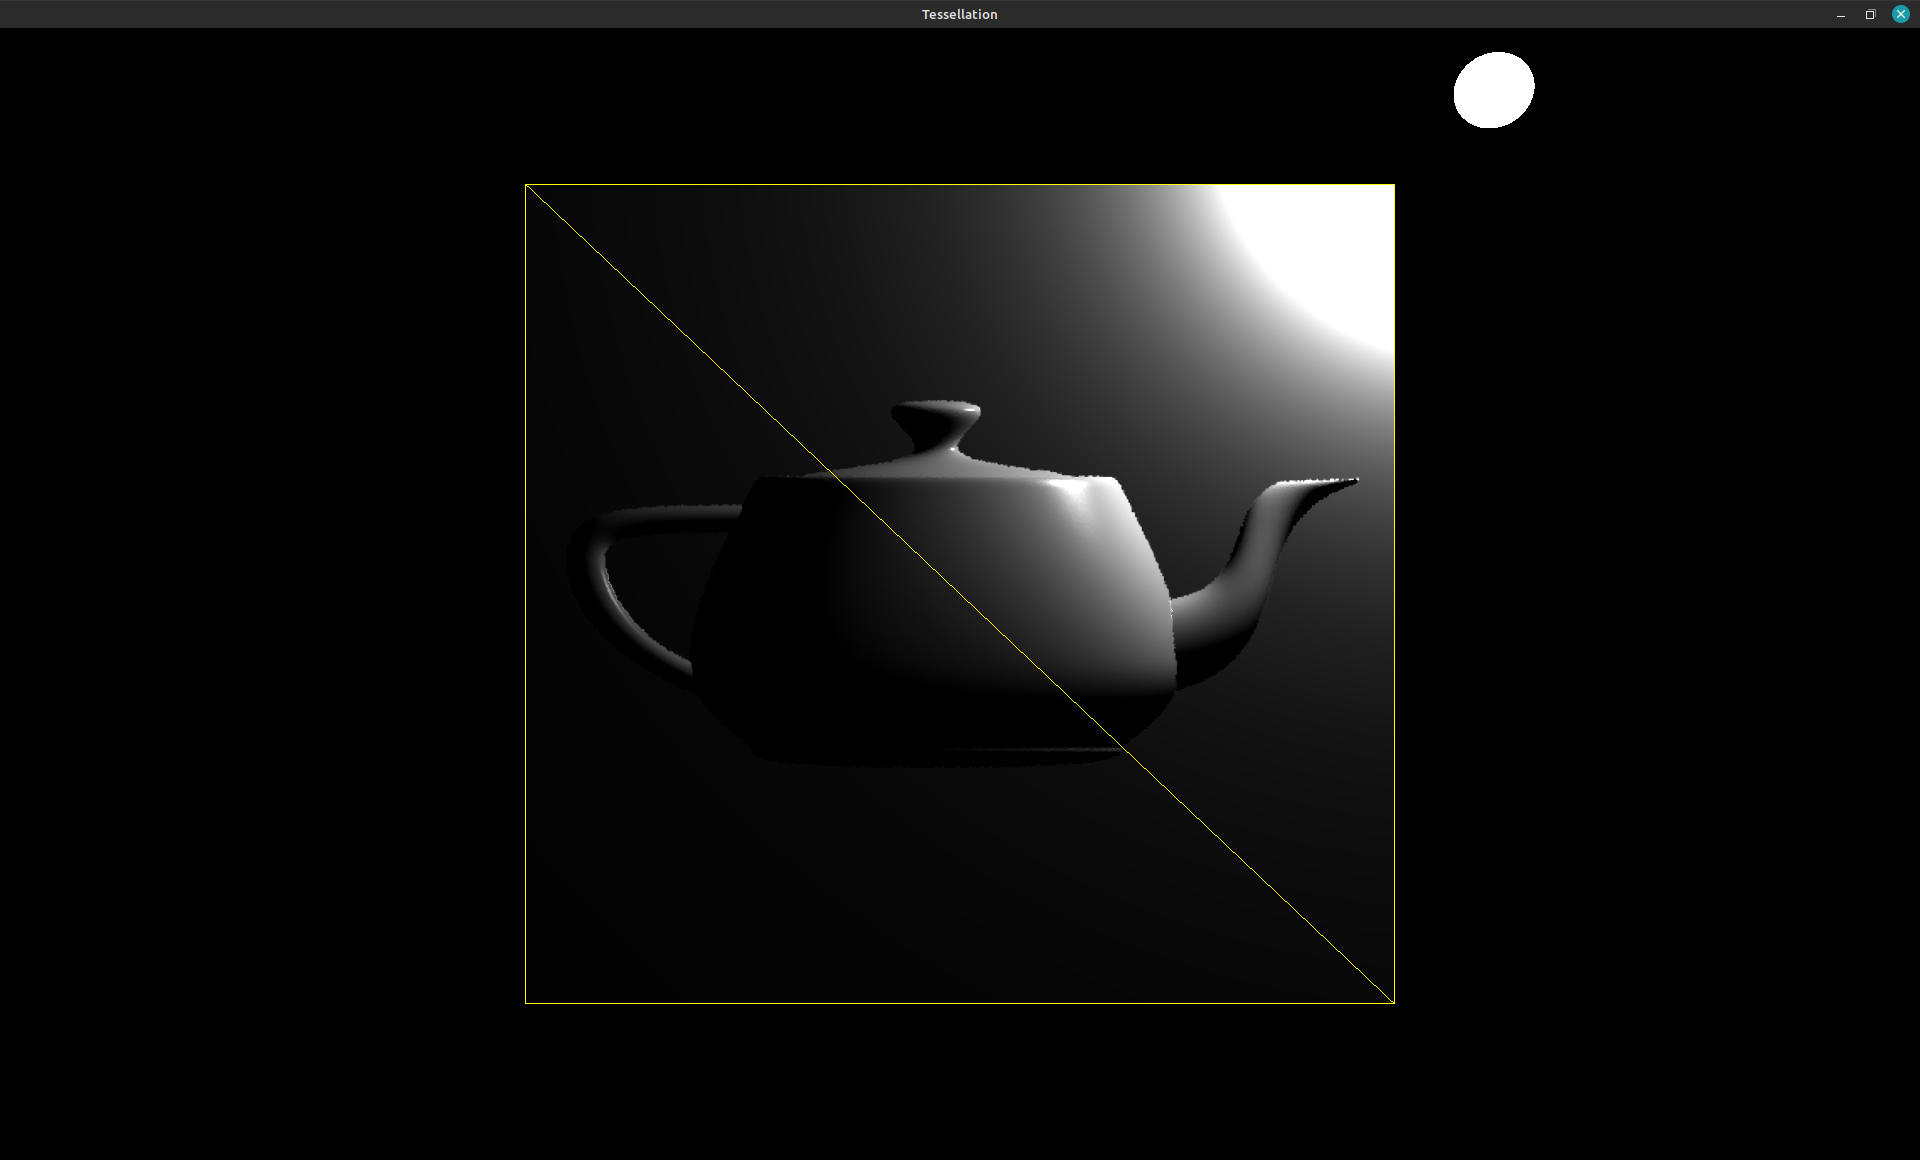
\includegraphics[width=0.7\textwidth]{images/normalTriangulation.png}\\
I didn't move the line segments closer to the camera, I just disabled depth testing.\\[2mm]
Next I added tessellation shaders to the triangulation shaders:\\
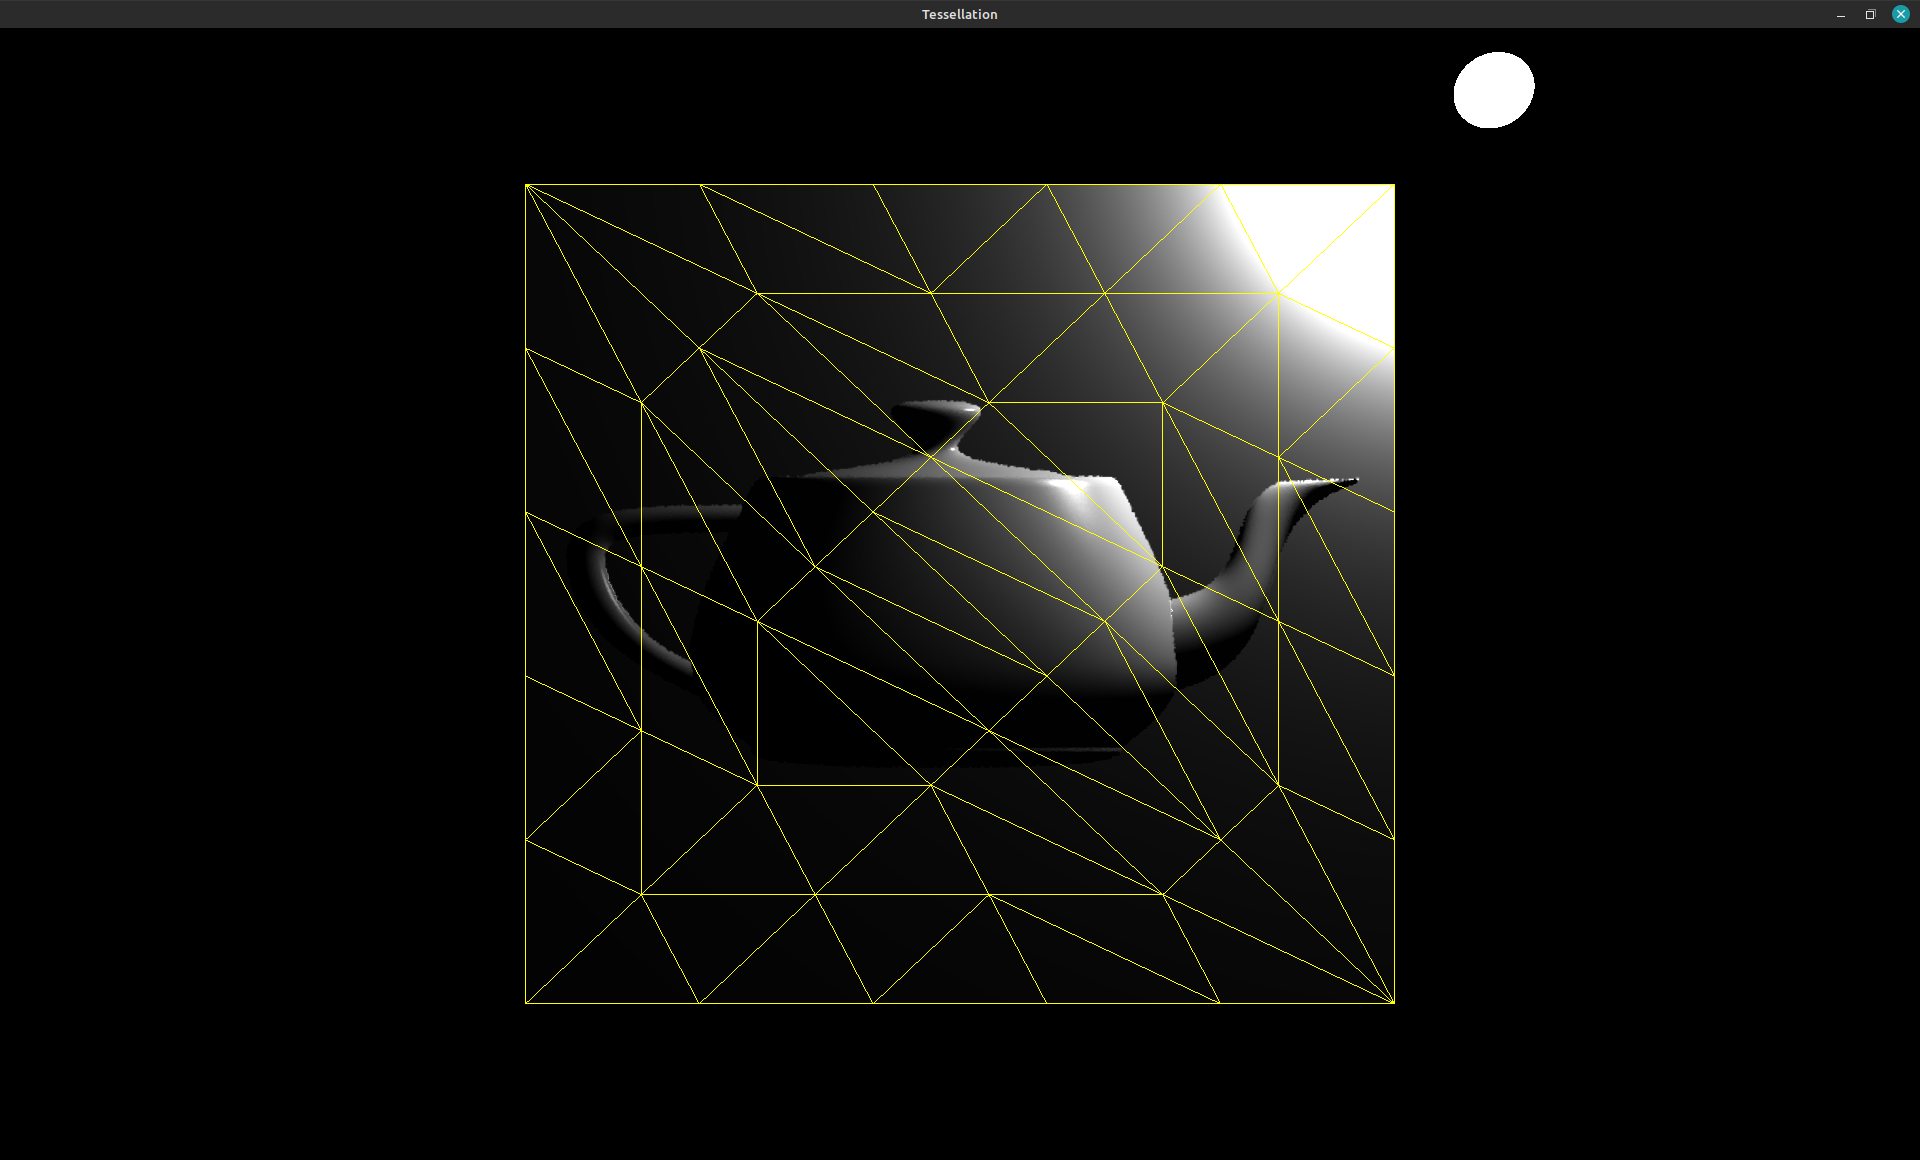
\includegraphics[width=0.7\textwidth]{images/triangulationTessellation.png}\\[2mm]
Next I added the controls using the arrow keys:\\
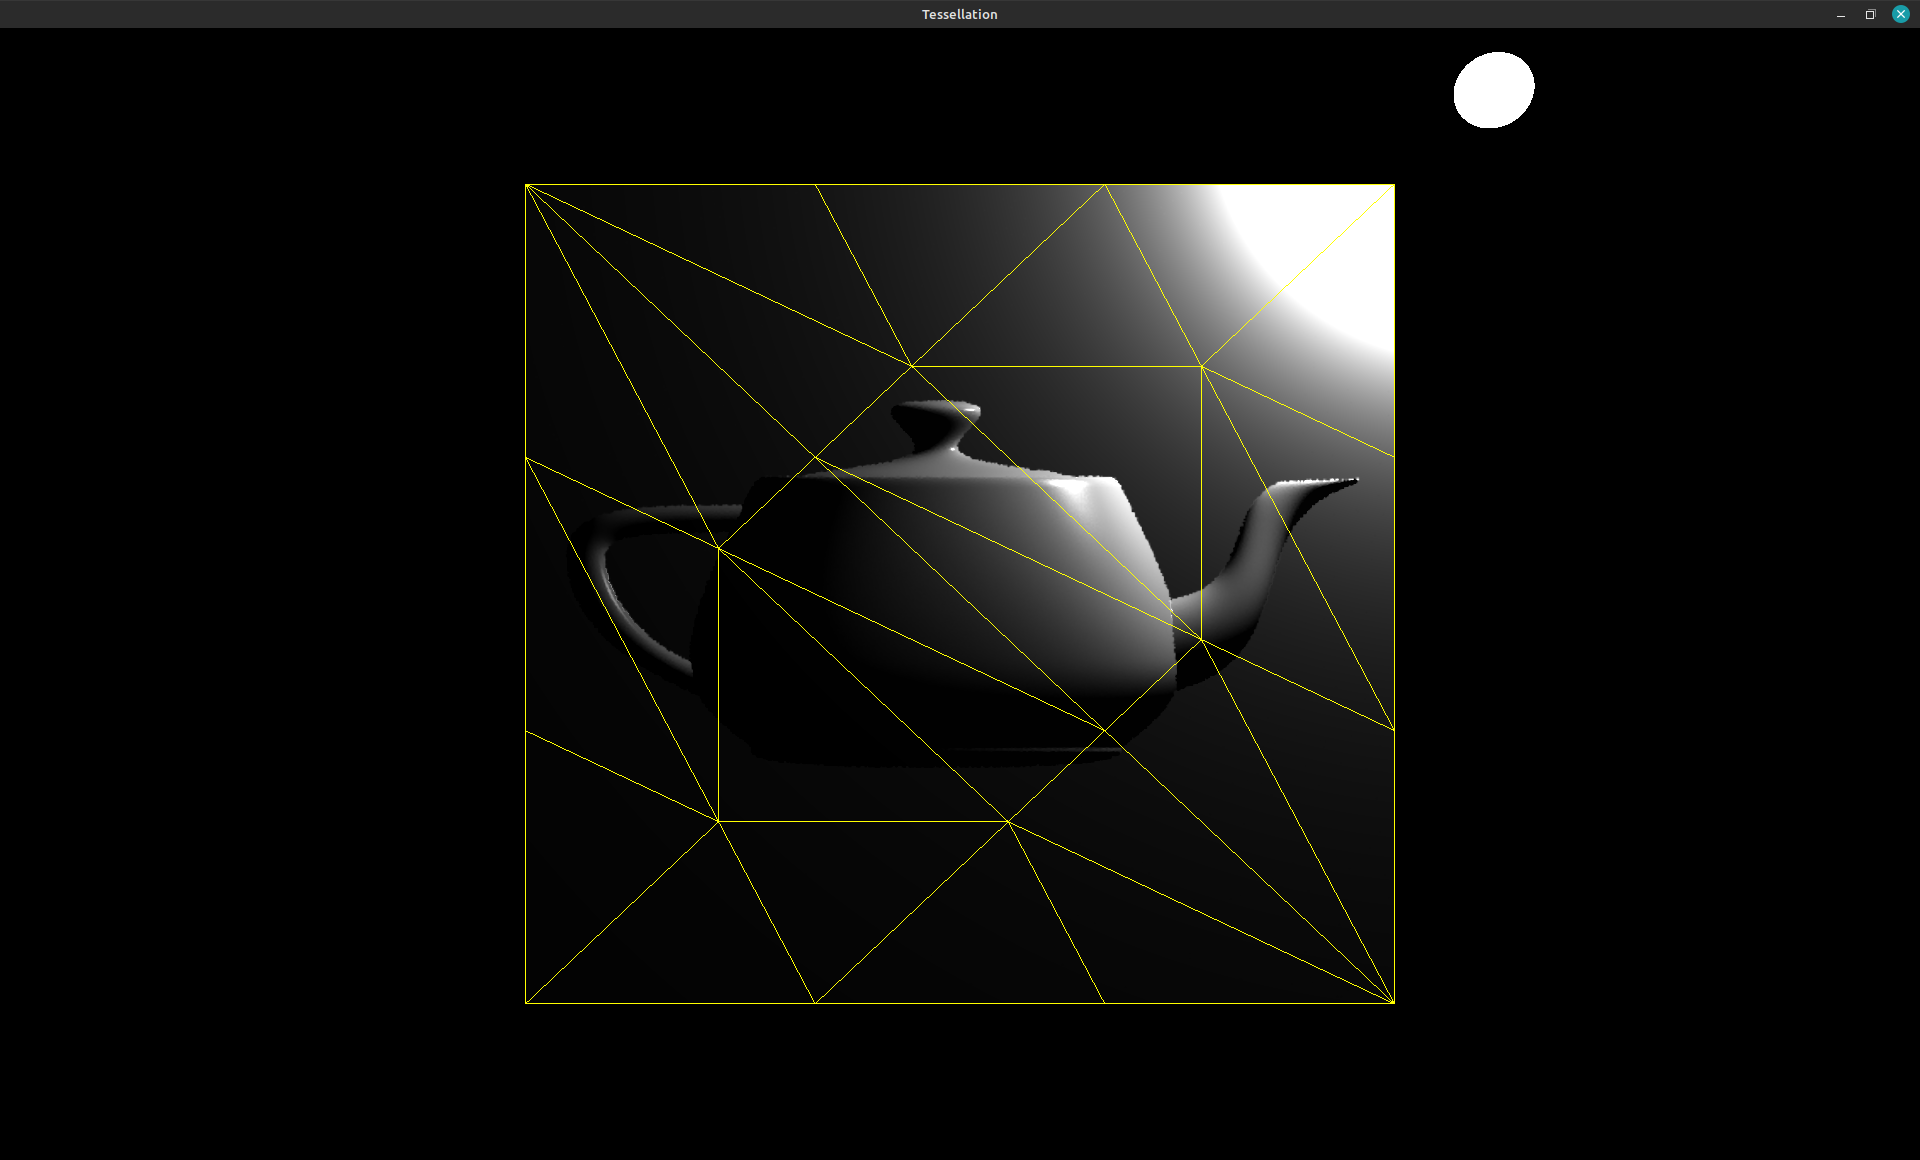
\includegraphics[width=0.4\textwidth]{images/tessLevel4Triangulation.png}
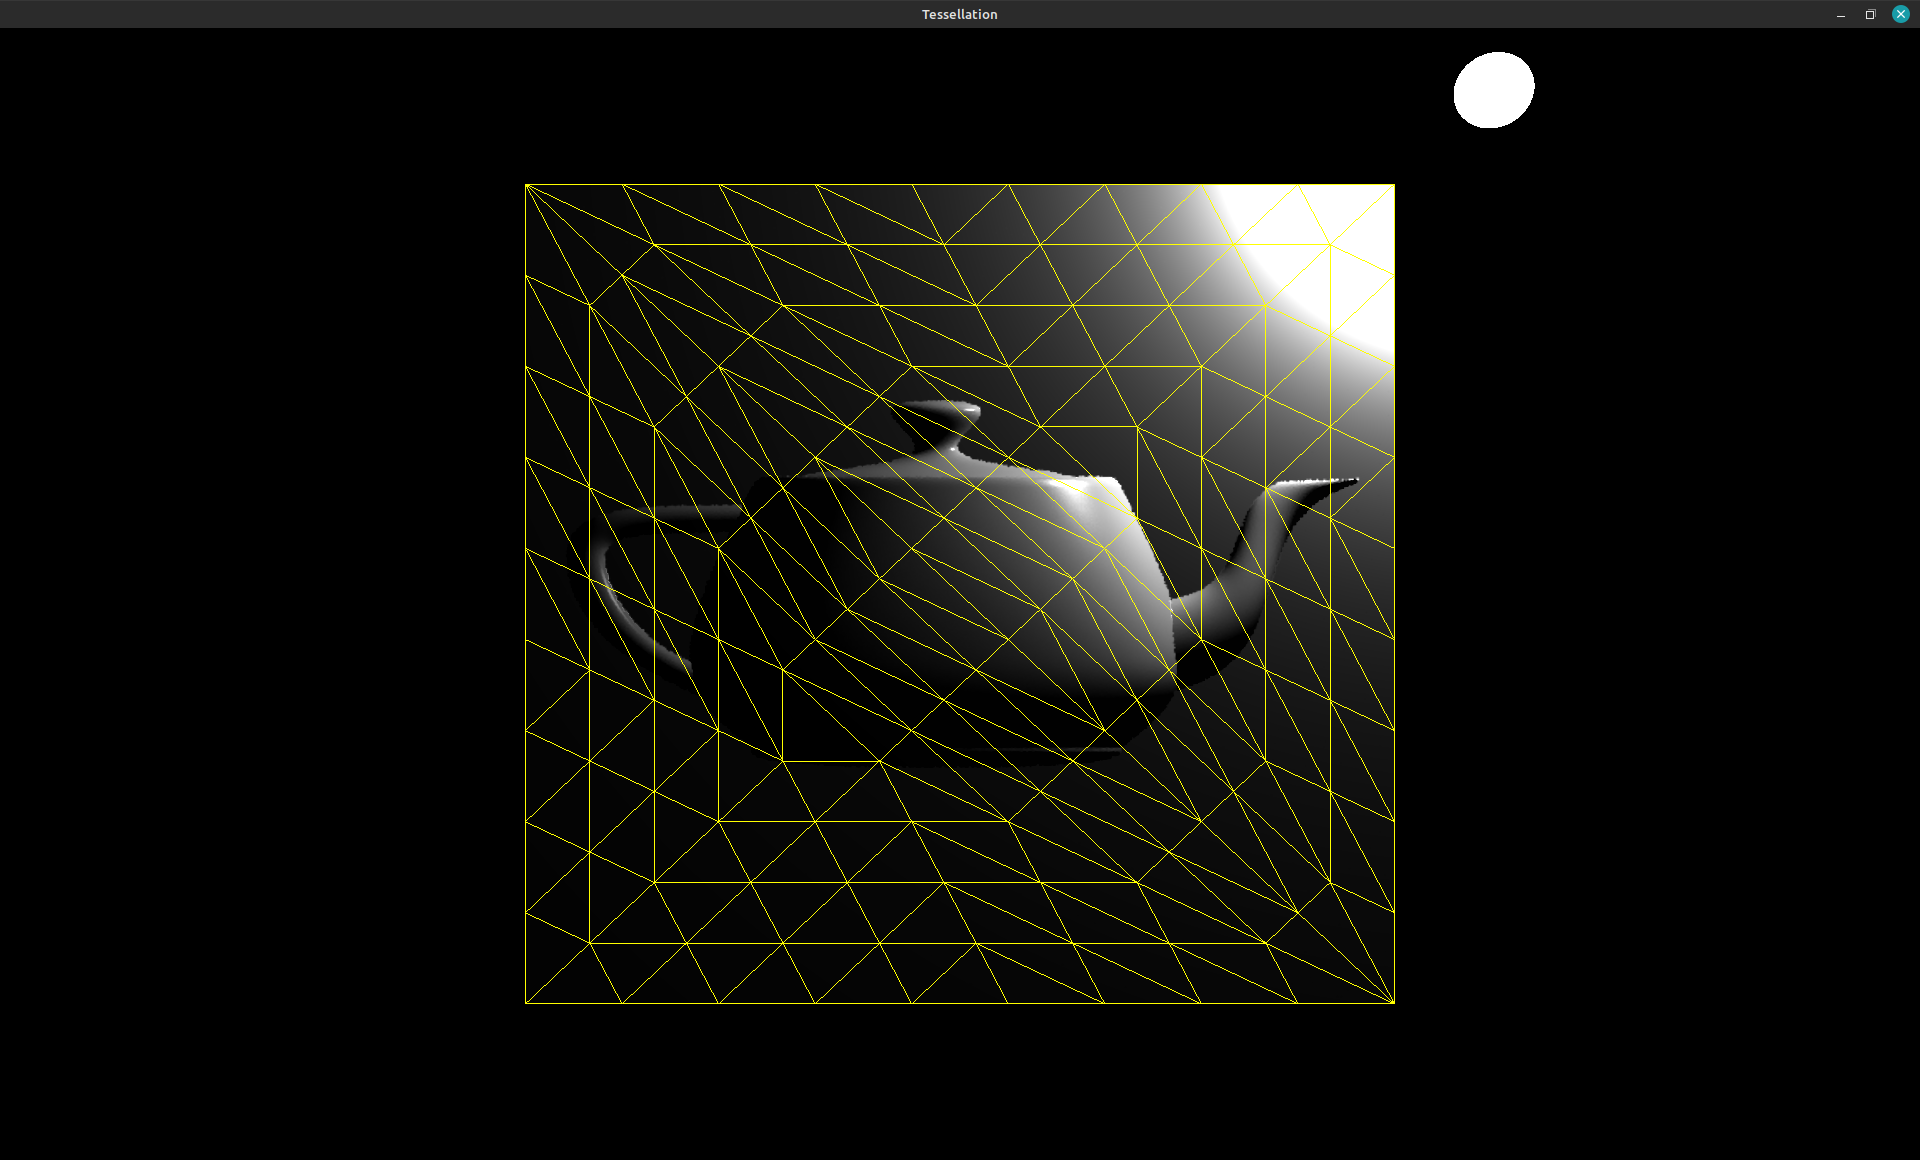
\includegraphics[width=0.4\textwidth]{images/tessLevel9Triangulation.png}\\[2mm]
Next I got the displacement map working for just the triangulation since that seemed simpler to start with:\\
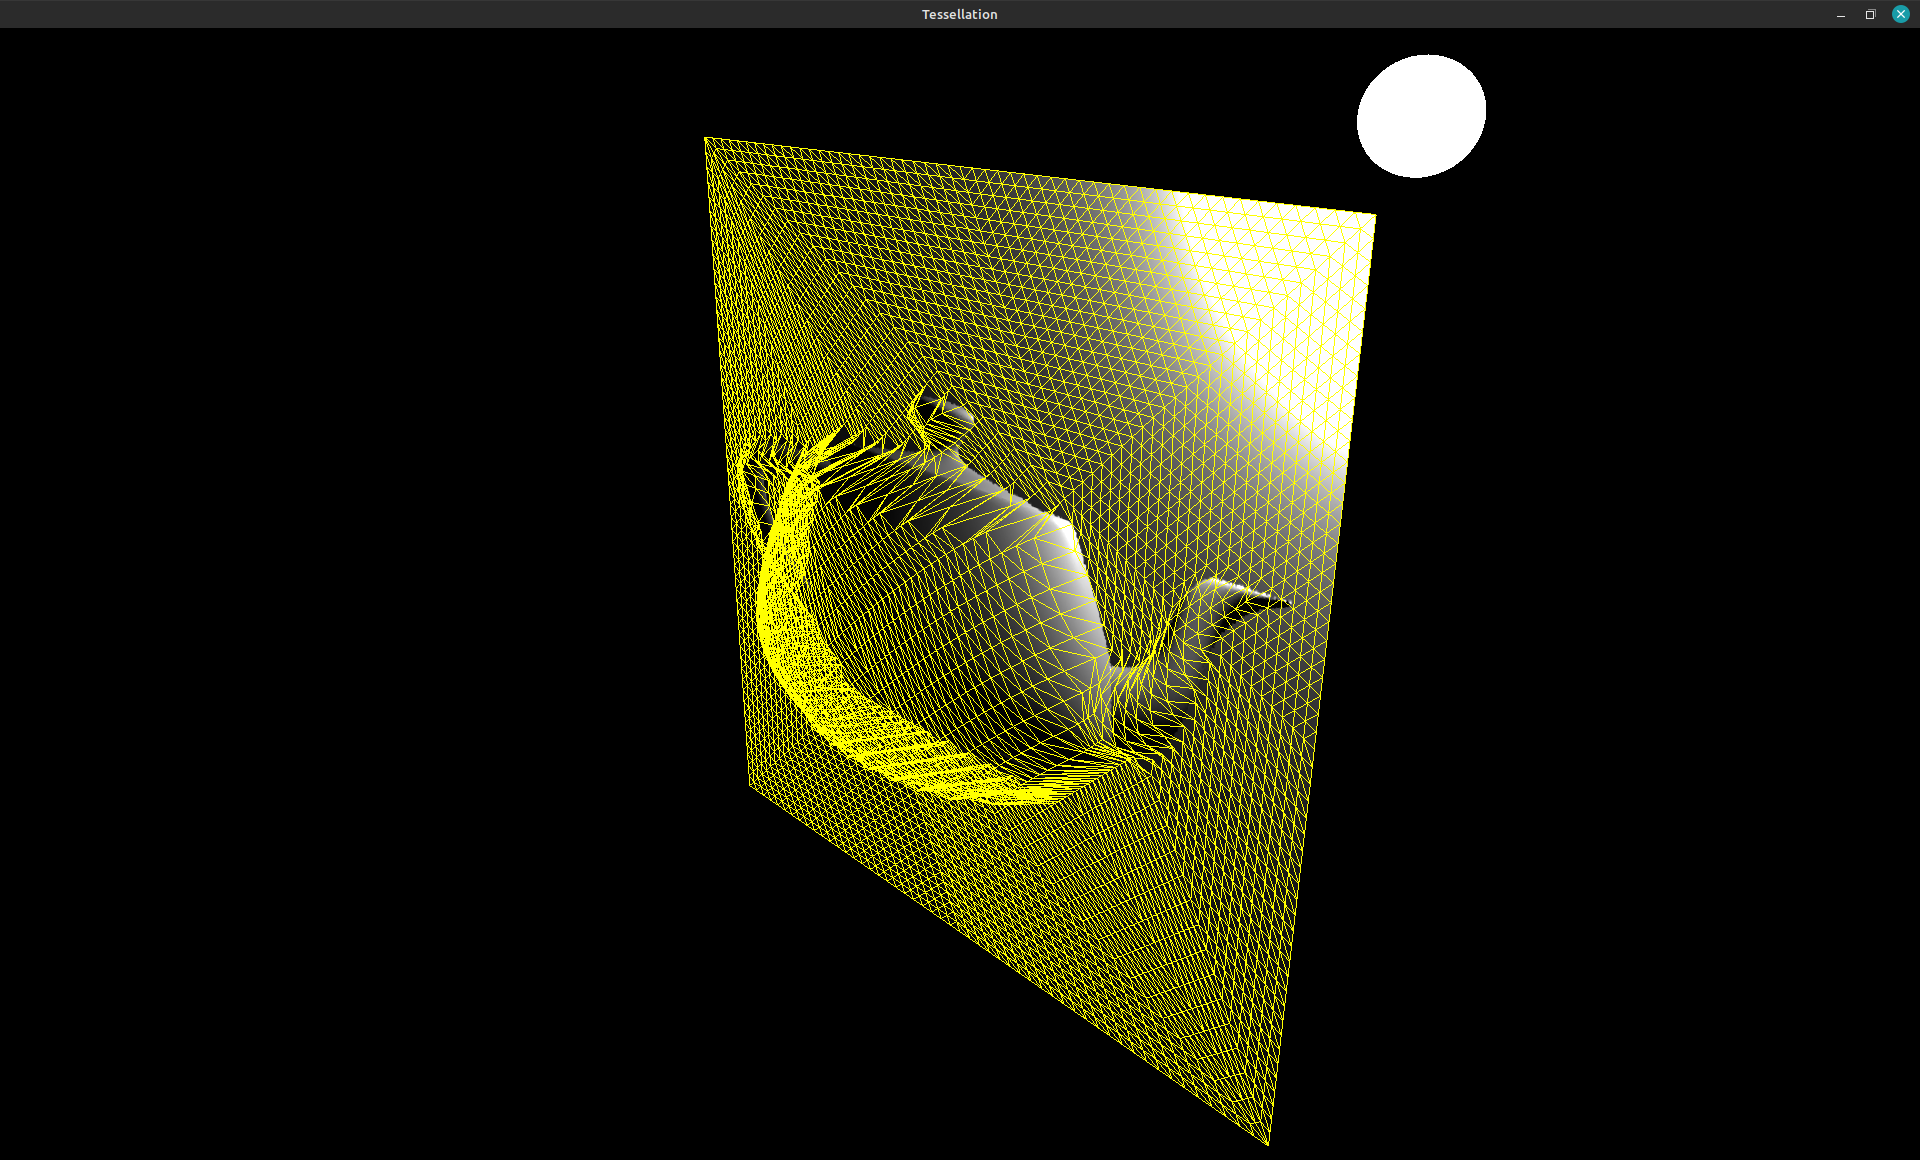
\includegraphics[width=0.7\textwidth]{images/displacementTriangulation.png}\\[2mm]
Next, I applied this to the main shader:\\
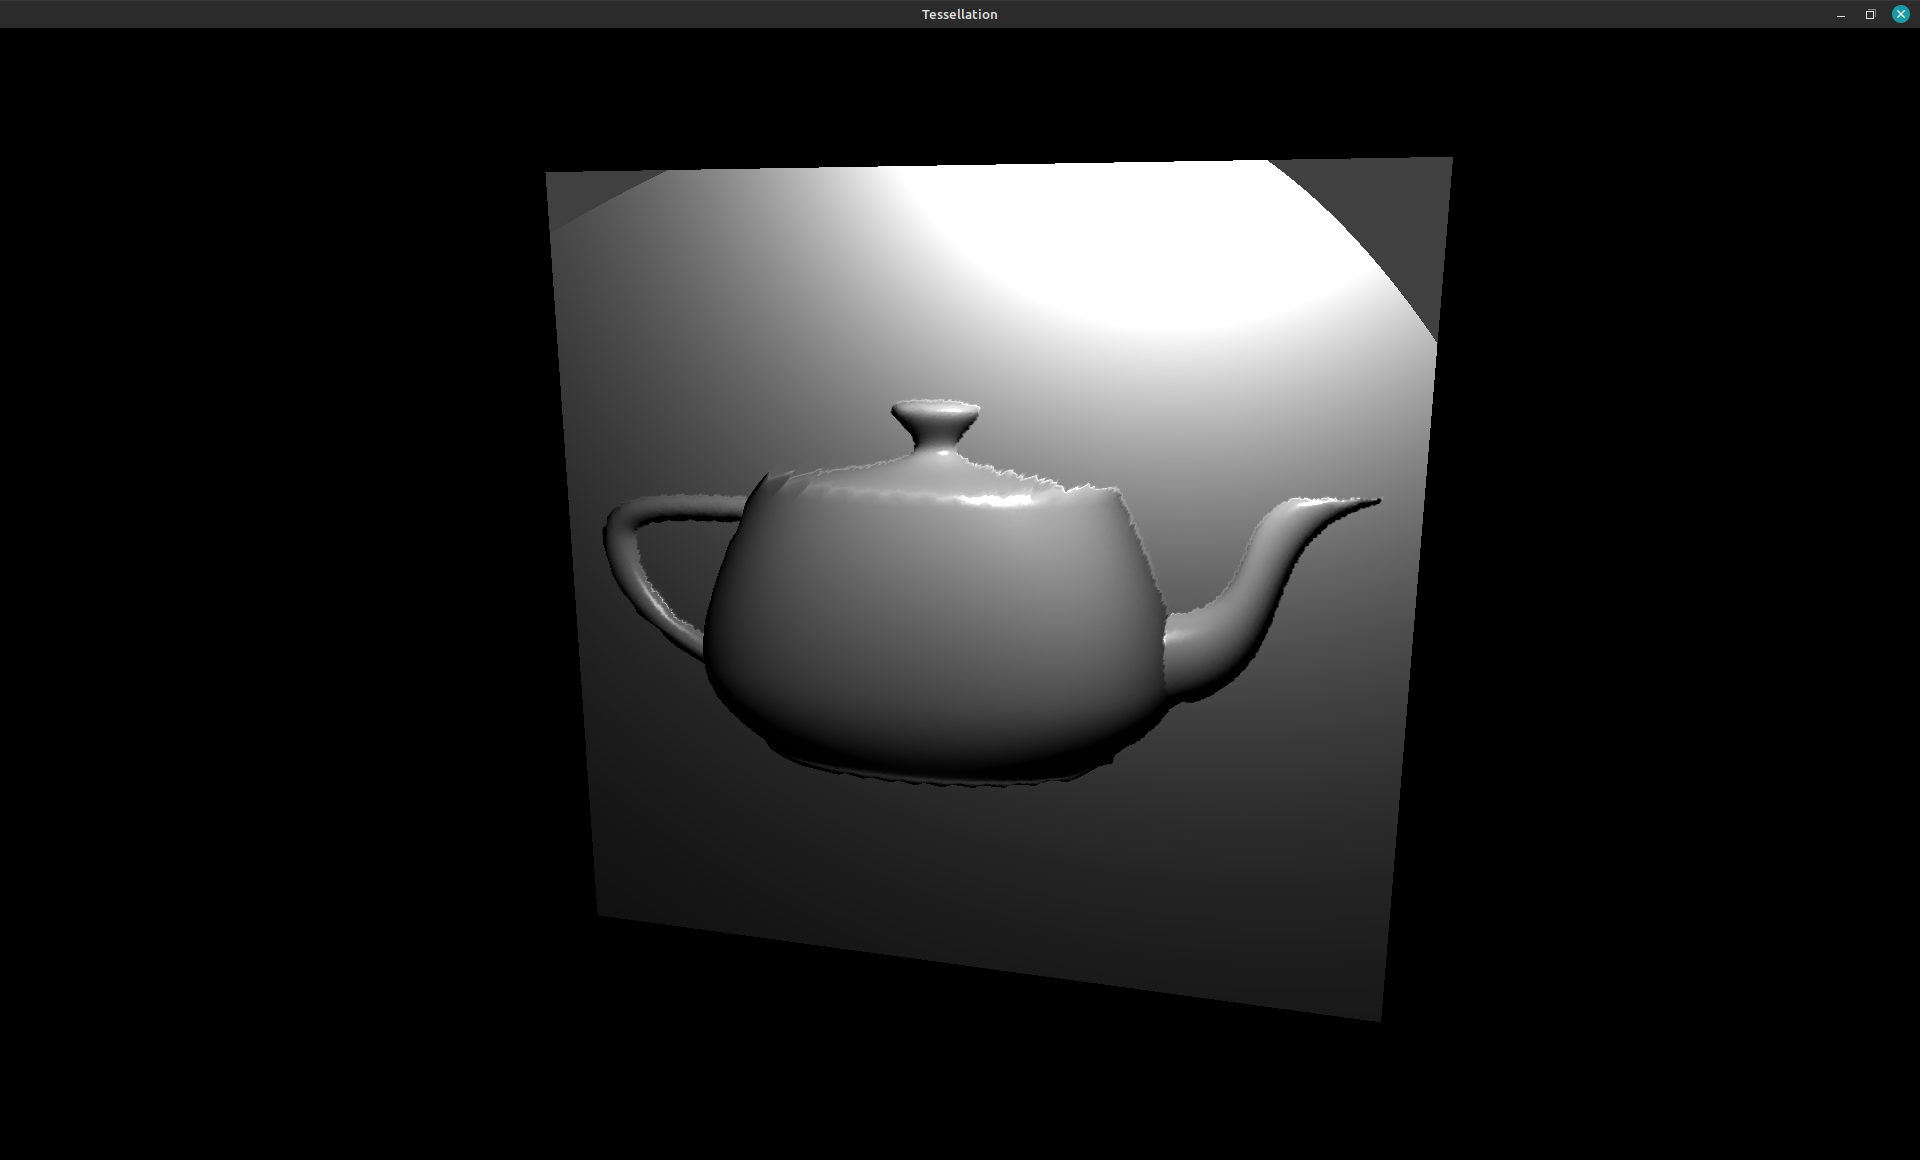
\includegraphics[width=0.7\textwidth]{images/displacementMapFirstAttempt.png}\\
What I noticed is that the edges seem a little jagged.\\[2mm]
Next I did the shadow mapping:\\
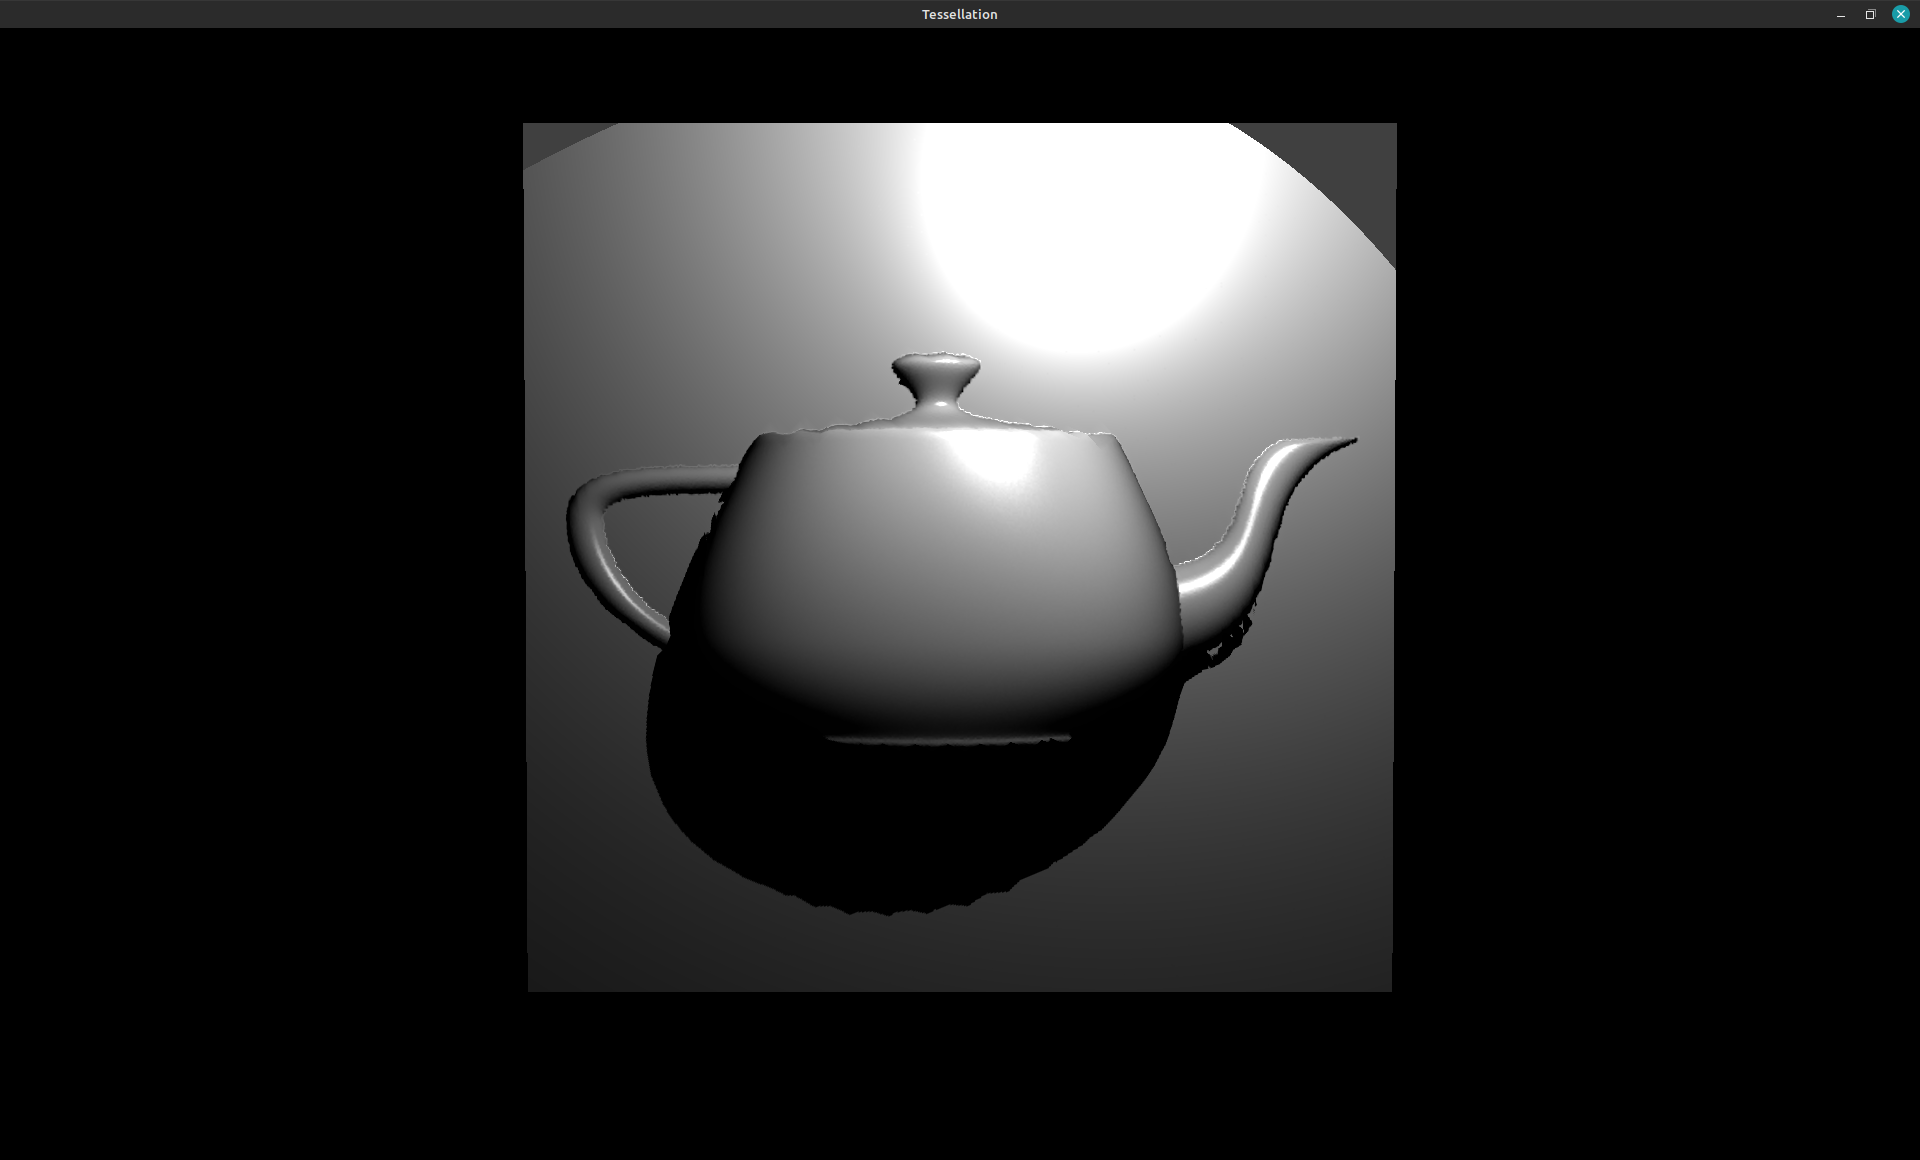
\includegraphics[width=0.7\textwidth]{images/jaggedShadows.png}\\[2mm]
Finally I decided to fix the jagged edges by tessellating everything into quads instead of triangles:\\
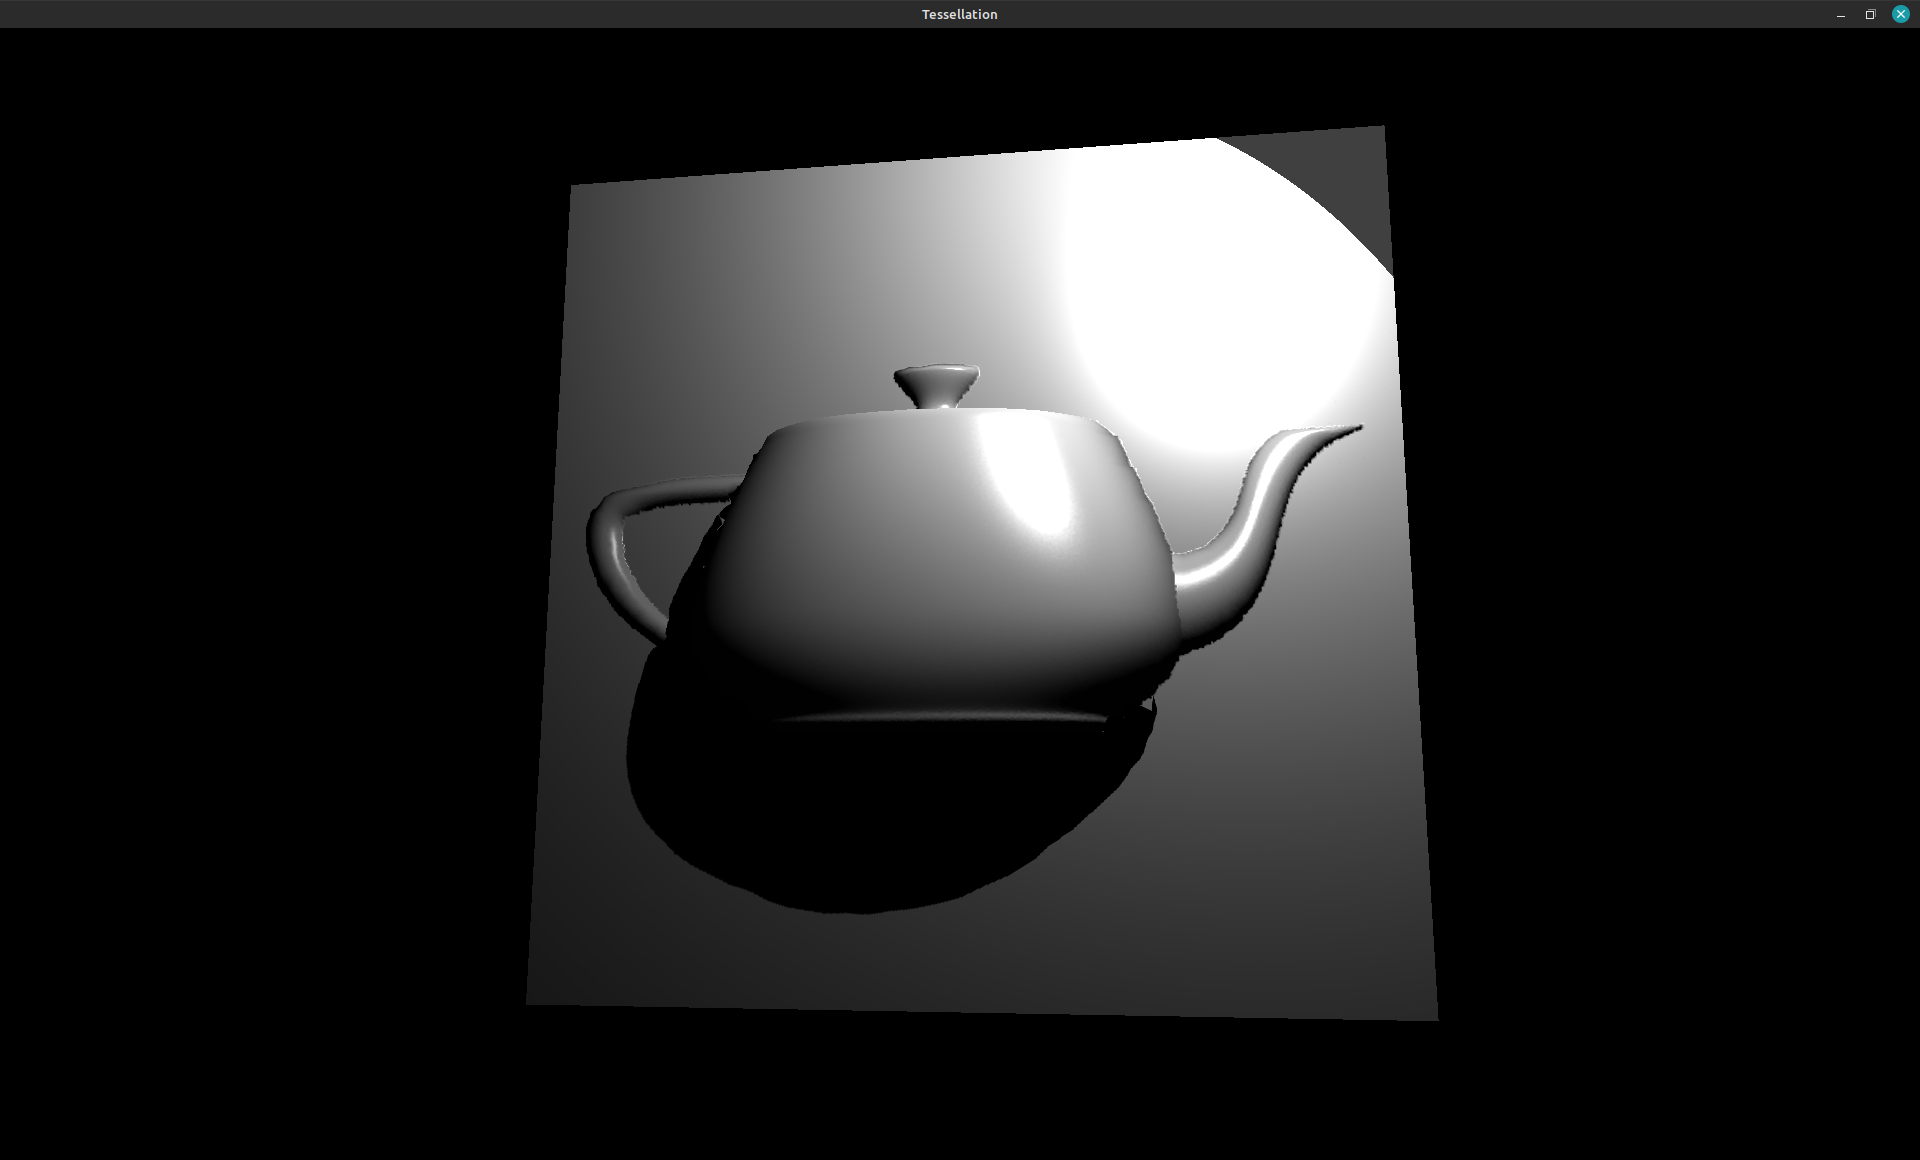
\includegraphics[width=0.4\textwidth]{images/smootherShadows.png}
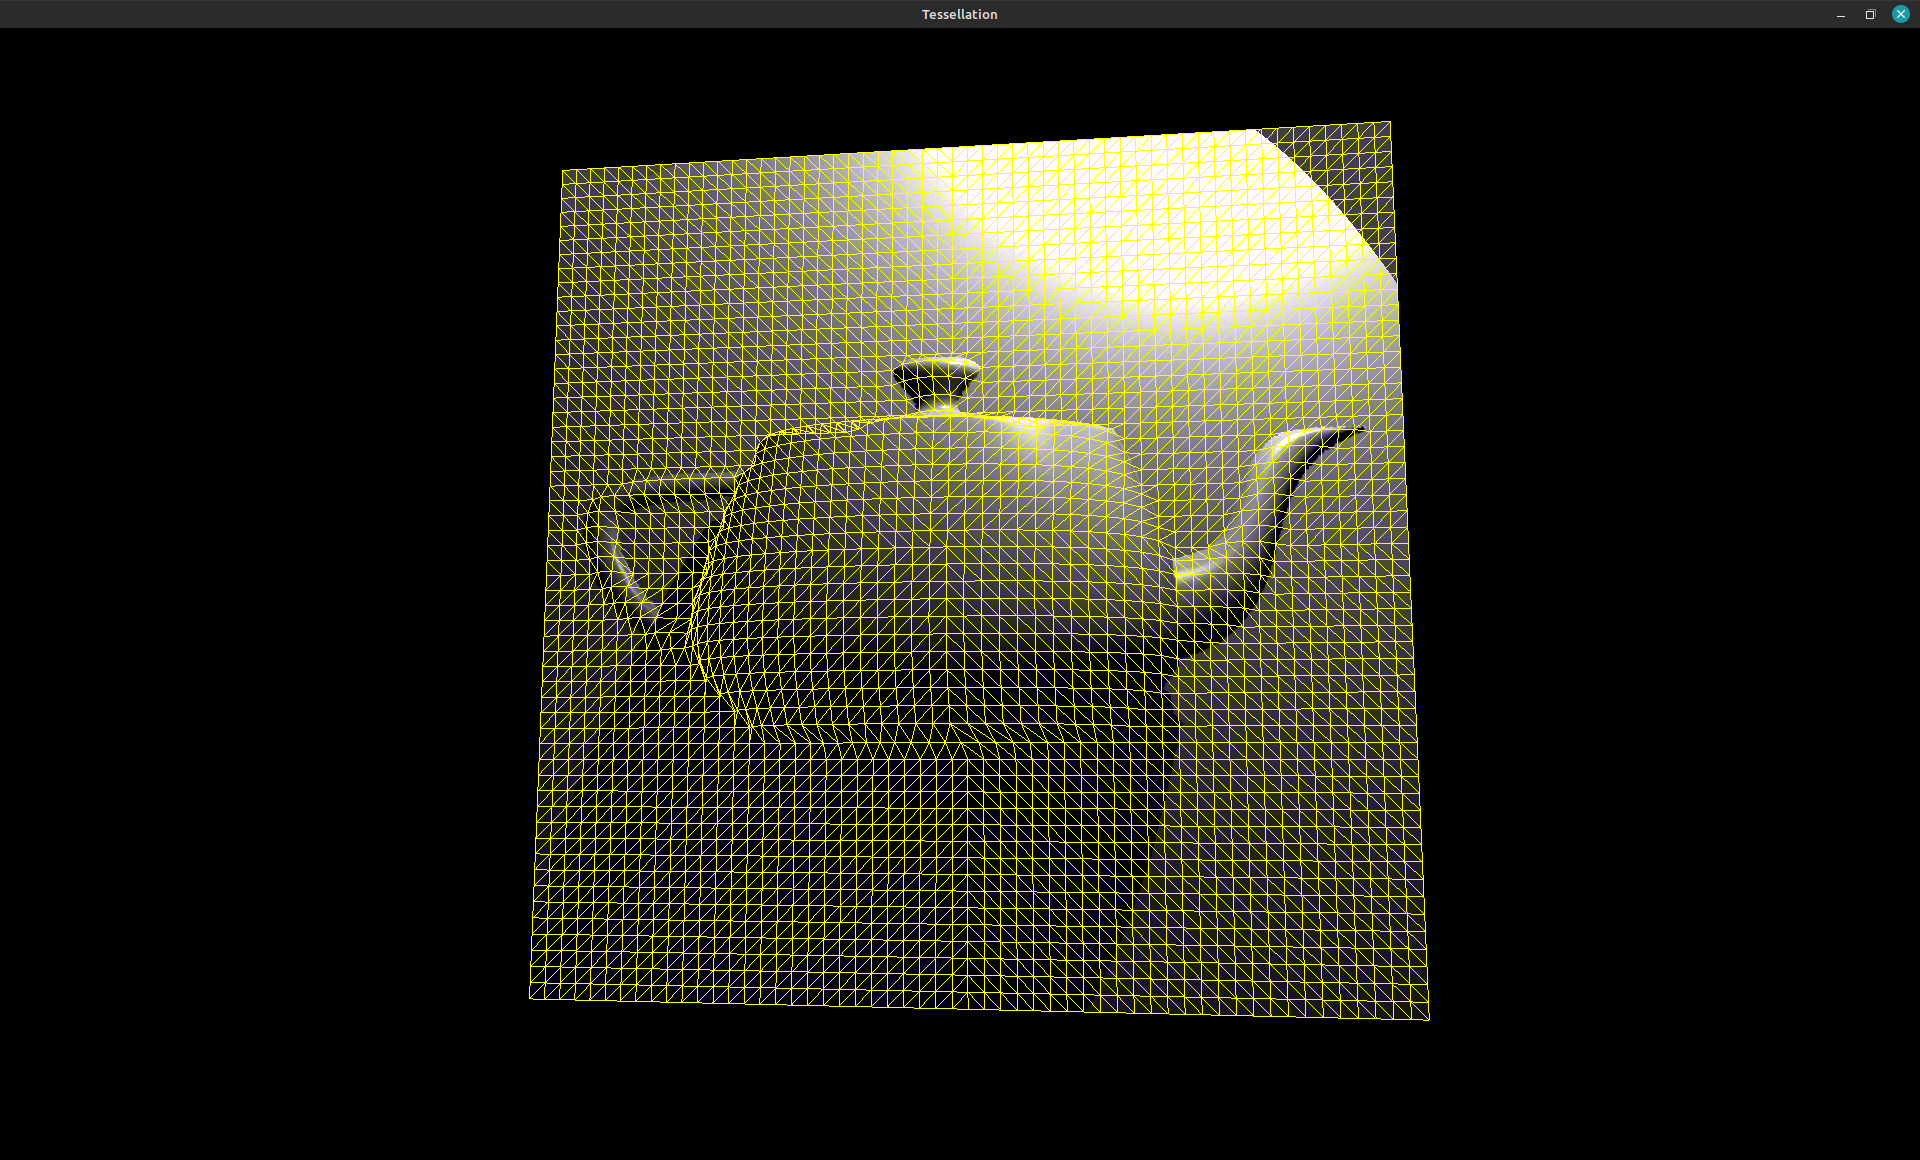
\includegraphics[width=0.4\textwidth]{images/quads.png}\\

\section*{6610 requirements and how to run}
I run this on Linux Mint using \texttt{glfw}, \texttt{glew}, \texttt{cyCore}, and \texttt{lodepng}.\\
To run this, go into the build directory and run:\\
\texttt{cmake ..}\\
\texttt{make}\\
\texttt{./main ../assets/teapot\_normal.png ../assets/teapot\_disp.png}\\
or\\
\texttt{./main ../assets/teapot\_normal.png}\\
if you just want to use normal maps.\\[2mm]
You can also just run:\\
\texttt{./main}\\
Which is equivalent to \texttt{./main ../assets/teapot\_normal.png ../assets/teapot\_disp.png}\\
since I got tired of typing the command line arguments everytime.

\end{document}

